% Source-backed analysis update assembled from:
%   ../docs/ml_results.md
%   ../docs/progress.md
%   ../docs/roadmap.md
%   ../Analysis_CODES/docs/ppref_x_reweighted_working_points.md
%   ../Analysis_CODES/docs/pbpb24_psi2s_selection_mass_scan.md
\documentclass[11pt,aspectratio=169]{beamer}

\usetheme{Madrid}
\usecolortheme{default}
\setbeamertemplate{navigation symbols}{}
\setbeamertemplate{footline}[frame number]

\usepackage{booktabs}
\usepackage{graphicx}
\usepackage{tikz}
\usetikzlibrary{arrows.meta,positioning}
\input{beamer_setup.tex}

% Optional fast single-frame build, e.g.:
%   bash fastcompile_frame.sh p18
\ifdefined\onlyframes
  \expandafter\includeonlyframes\expandafter{\onlyframes}
\fi

\definecolor{positive}{HTML}{0173B2}
\definecolor{negative}{HTML}{DE8F05}
\definecolor{emphasis}{HTML}{027A5A}
\definecolor{neutral}{HTML}{666666}
\definecolor{panelbg}{HTML}{F4F6F8}
\setbeamercolor{structure}{fg=positive}
\setbeamercolor{block title}{fg=white,bg=positive}
\setbeamercolor{block body}{fg=black,bg=positive!8}
\setbeamercolor{block title alerted}{fg=white,bg=negative}
\setbeamercolor{block body alerted}{fg=black,bg=negative!10}
\setbeamercolor{block title example}{fg=white,bg=emphasis}
\setbeamercolor{block body example}{fg=black,bg=emphasis!8}
\newcommand{\pos}[1]{\textcolor{positive}{#1}}
\newcommand{\con}[1]{\textcolor{negative}{#1}}
\newcommand{\HL}[1]{\textcolor{emphasis}{#1}}
\newcommand{\muted}[1]{\textcolor{neutral}{#1}}

\title[X(3872) Analysis Update]{X(3872) Analysis Update}
\subtitle{From \texorpdfstring{\psiP}{psi(2S)} reweighting to the current PbPb strategy}
\author{%
  Henrique Legoinha, \underline{Lekai Yao}, Nuno Leonardo, Zhen Hu\\[0.45em]
  2026.8.5%
}
\institute{}
\date{%
  \includegraphics[height=1.653cm]{figures/symbols/CERN.png}\hspace{0.30cm}%
  \includegraphics[height=1.653cm]{figures/symbols/CMS.png}\hspace{0.30cm}%
  \includegraphics[height=1.653cm]{figures/symbols/LIP.png}\hspace{0.30cm}%
  \includegraphics[height=1.653cm]{figures/symbols/LU.png}\hspace{0.30cm}%
  \includegraphics[height=1.653cm]{figures/symbols/THU.png}%
}

\begin{document}

\begin{frame}[plain,label=p1]
  \titlepage
\end{frame}

\begin{frame}{Recap: where the previous update stopped}
  \centering
  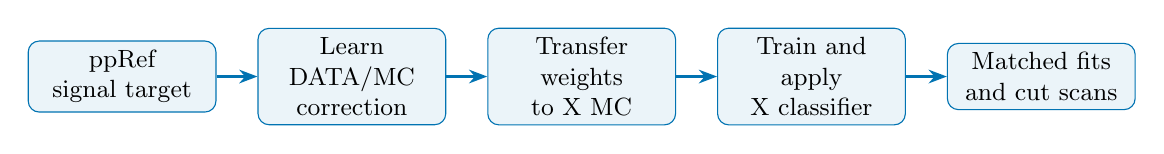
\begin{tikzpicture}[
    box/.style={
      draw=positive,
      rounded corners,
      fill=positive!8,
      minimum height=0.82cm,
      text width=2.15cm,
      align=center,
      font=\small
    },
    arr/.style={-{Stealth},thick,positive}
  ]
    \node[box] (signal) {ppRef \psiP\\signal target};
    \node[box,right=0.52cm of signal] (rw) {Learn DATA/MC\\correction};
    \node[box,right=0.52cm of rw] (apply) {Transfer weights\\to X MC};
    \node[box,right=0.52cm of apply] (ml) {Train and apply\\X classifier};
    \node[box,right=0.52cm of ml] (fit) {Matched fits\\and cut scans};
    \draw[arr] (signal) -- (rw);
    \draw[arr] (rw) -- (apply);
    \draw[arr] (apply) -- (ml);
    \draw[arr] (ml) -- (fit);
  \end{tikzpicture}

  \vspace{0.8em}
  \begin{columns}[T]
    \begin{column}{0.48\textwidth}
      \begin{exampleblock}{ppRef: end-to-end prototype completed}
        \begin{itemize}
          \item Signal extraction, reweighting, X MC application
          \item Weighted/unweighted ML, matched fits, cut scans
          \item Technical workflow established; physics choice not frozen
        \end{itemize}
      \end{exampleblock}
    \end{column}
    \begin{column}{0.48\textwidth}
      \begin{alertblock}{PbPb: no reliable \texorpdfstring{\psiP}{psi(2S)} target}
        \begin{itemize}
          \item Cumulative selections and S2/S3 fits checked
          \item No sufficiently robust peak for a signed-sWeight target
          \item PbPb-specific reweighting could not start from this route
        \end{itemize}
      \end{alertblock}
    \end{column}
  \end{columns}

  \vfill
  \centering\HL{This update revisits the ppRef assumptions before choosing a PbPb strategy.}
\end{frame}

\begin{frame}{Comments postponed}
  \vspace{4pt}
  \begin{center}
    \footnotesize
    \begin{tabular}{p{3.5cm}p{9.1cm}}
      \toprule
      Comment & Reason for postponement \\
      \midrule
      Use ML AUC to decide whether more inputs are better? &
      MC-based AUC is not a reliable standalone criterion for variable inclusion. \\
      \addlinespace
      Add \texttt{B\_alpha}? &
      Not a current bottleneck; no new training or validation in this update. \\
      \addlinespace
      Add muon variables? &
      Revisit only after the reweighting and transfer strategy is defined. \\
      \addlinespace
      Move \texttt{BQvalue} into the fiducial region? &
      A broad bias question requiring a dedicated selection and systematic study. \\
      \bottomrule
    \end{tabular}
  \end{center}

  \vspace{0.35em}
  \begin{columns}[T]
    \begin{column}{0.48\textwidth}
      \centering
      \textbf{What AUC can tell us}\\[0.2em]
      \footnotesize Separation power on the simulated validation sample.
    \end{column}
    \begin{column}{0.48\textwidth}
      \centering
      \textbf{What it cannot establish}\\[0.2em]
      \footnotesize DATA modelling, transfer closure, or final analysis robustness.
    \end{column}
  \end{columns}

  \vfill
  \centering\itshape
  Feature expansion is paused until the correction strategy and validation scope are fixed.
\end{frame}

\begin{frame}{What does AUC $=0.5$ mean here?}
  \begin{columns}[T]
    \begin{column}{0.58\textwidth}
      \centering
      \includegraphics[width=\textwidth,height=0.47\textheight,keepaspectratio]
      {../XGBoost/output/slides_evidence/a5_b1_b3_v1/b3/holdout_domain_classifier_auc.pdf}
    \end{column}
    \begin{column}{0.38\textwidth}
      \small
      \textbf{This diagnostic}\\[-0.2em]
      \begin{itemize}
        \item Classifies \textbf{DATA target vs. MC domain}
        \item Positive: signed-sWeighted \psiP DATA
        \item Negative: \psiP MC before/after R5 correction
      \end{itemize}
      \vspace{0.2em}
      \textbf{Different from ML AUC}\\[0.15em]
      Signal-vs-background AUC should be high; domain AUC should approach 0.5 after correction.

      \vspace{0.35em}
      \textbf{Five holdout splits after reweighting:}\\[0.2em]
      range $0.5066$--$0.5285$; mean $0.5217$.

    \end{column}
  \end{columns}
\end{frame}

\begin{frame}{From the KS test to a signed-weight KS-like distance}
  \begin{columns}[T]
    \begin{column}{0.48\textwidth}
      \textbf{Standard two-sample KS test}
        \small\\[-0.3em]
        \[
          D_{n,m}=\sup_x\left|F_n(x)-G_m(x)\right|.
        \]
        \begin{itemize}
          \item Unweighted, monotonic empirical CDFs
          \item A KS p-value follows under standard assumptions
        \end{itemize}
    \end{column}
    \begin{column}{0.48\textwidth}
      \textbf{Our signed-weight distance}
        \small\\[-0.3em]
        \[
          D=\sup_x\left|F_{\rm MC}(x)-F_{\rm target}^{\rm signed}(x)\right|.
        \]
        \begin{itemize}
          \item Negative sWeights are retained
          \item Signed CDF may decrease or leave $[0,1]$
          \item Descriptive effect size, not a KS p-value
        \end{itemize}
    \end{column}
  \end{columns}

  \vspace{0.4em}
  \small
  \textbf{Completed bootstrap study:} 500 paired replicas; resample DATA/MC, retain signed
  event weights, retrain each reweighter, and evaluate an independent holdout.

  \vspace{0.35em}
  \begin{center}
    \begin{tabular}{ll}
      \toprule
      Covered & Not covered \\
      \midrule
      Finite-event fluctuations; retraining & Fit model/range; sWeight construction \\
      \bottomrule
    \end{tabular}
  \end{center}

  \vfill
  \centering\itshape
  Later recipe scans use point estimates only; the bootstrap is not repeated by default.
\end{frame}

\begin{frame}{SHAP importance in the new nominal workflow}
  \begin{columns}[T]
    \begin{column}{0.49\textwidth}
      \centering
      \vspace{-0.45em}
      \textbf{R6range2-weighted classifier}\\[0.15em]
      \includegraphics[width=\textwidth,height=0.46\textheight,keepaspectratio]
      {../XGBoost/output/slides_evidence/a5_b1_b3_v1/a5/weighted/shap_cumulative.pdf}
    \end{column}
    \begin{column}{0.49\textwidth}
      \centering
      \vspace{-0.45em}
      \textbf{Unweighted classifier}\\[0.15em]
      \includegraphics[width=\textwidth,height=0.46\textheight,keepaspectratio]
      {../XGBoost/output/slides_evidence/a5_b1_b3_v1/a5/unweighted/shap_cumulative.pdf}
    \end{column}
  \end{columns}

  \vspace{0.25em}
  \small
  \textbf{R6range2 correction used by this artifact:}
  \texttt{Bcos\_dtheta}$\in[-1,1]$,
  \texttt{Btktkpt}$\in[2,10]$,
  \texttt{Bchi2Prob}$\in[0,1]$,
  \texttt{Btrk2Pt}$\in[0.5,4.5]$,
  \texttt{Btrk1Pt}$\in[0.5,4.5]$,
  \texttt{Btrk1dR}$\in[0,0.5]$.

  \vfill
  \centering\HL{New nominal chain: ppRef X fit $\to$ reweighting $\to$
  PbPb weighted-vs-unweighted ML comparison.}
\end{frame}

\begin{frame}{SHAP importance versus ppRef X closure}
  \centering
  \small
  \setlength{\tabcolsep}{5pt}
  \begin{tabular}{lrrr}
    \toprule
    Variable & SHAP fraction: unweighted $\to$ weighted & KS-like: before $\to$ after & Pattern \\
    \midrule
    \texttt{Btrk1dR}      & 19.33\% $\to$ 31.34\% & 0.051 $\to$ 0.039 & importance rises \\
    \texttt{Btktkpt}      & 33.94\% $\to$ 22.10\% & 0.242 $\to$ 0.037 & both decrease \\
    \texttt{Bchi2Prob}    & 16.22\% $\to$ 12.47\% & 0.123 $\to$ 0.032 & both decrease \\
    \texttt{Bcos\_dtheta} &  7.57\% $\to$ 10.63\% & 0.260 $\to$ 0.040 & importance rises \\
    \texttt{Btrk2Pt}      &  9.29\% $\to$  9.94\% & 0.093 $\to$ 0.017 & nearly stable \\
    \texttt{Btrk1Pt}      &  9.72\% $\to$  9.06\% & 0.176 $\to$ 0.043 & mild decrease \\
    \bottomrule
  \end{tabular}

  \vfill
  \centering\HL{Corrected variables remain dominant, but no simple monotonic SHAP--closure relation is observed.}

  \vspace{0.1em}
  \centering\small
  SHAP: PbPb classifiers; KS-like: ppRef X R6range2 closure. The comparison is qualitative.
\end{frame}

\begin{frame}{Why did the previous plot not show the maximum weight?}
  \begin{columns}[T]
    \begin{column}{0.49\textwidth}
      \centering
      \vspace{-0.45em}
      \textbf{Previous update}\\[0.15em]
      \includegraphics[width=\textwidth,height=0.48\textheight,keepaspectratio]
      {../XGBoost/output/reweighting/comparison_pp24_psi2s/weight_distributions_R3_R4_R5_R8.pdf}
    \end{column}
    \begin{column}{0.49\textwidth}
      \centering
      \vspace{-0.45em}
      \textbf{Corrected full-range view}\\[0.15em]
      \includegraphics[width=\textwidth,height=0.48\textheight,keepaspectratio]
      {../XGBoost/output/slides_evidence/a5_b1_b3_v1/b1/weight_distributions_full_range.pdf}
    \end{column}
  \end{columns}

  \vspace{0.35em}
  \begin{itemize}
    \item The previous histogram stopped at the \textbf{99.5\% positive-weight quantile};
      its legend nevertheless reported the true maximum.
    \item The corrected view spans the complete finite positive-weight range:
      the long tail is visible and the R8 maximum $=219.262$ is real.
  \end{itemize}

\end{frame}

\begin{frame}{How is the ppRef X validation target constructed?}
  \centering
  \small\textbf{Comment from the previous update:} compare the X sPlot target with
  \psiP-reweighted X MC and quantify the agreement with a KS-like distance.

  \vspace{0.2em}
  \begin{columns}[T]
    \begin{column}{0.43\textwidth}
      \centering
      \includegraphics[width=\textwidth,height=0.39\textheight,keepaspectratio]
      {../Analysis_CODES/fitER/results/ppRef_X_r5_fiducial_feasibility/diagnostics/mass_fit_components_pull.pdf}

      \footnotesize
      Technically accepted fit: status $=0$, covQual $=3$;\quad
      $N_X=3795\pm288$.
    \end{column}
    \begin{column}{0.49\textwidth}
      \footnotesize
      \textbf{Independent X target}\\[-0.2em]
      \begin{itemize}
        \item $7.5<p_T(B)<50$, $|y|<2.4$, \texttt{BQvalue}$<0.15$
        \item Yield-only sPlot refit; signed weights retained
        \item $N_{\rm eff}=393.74$ from 194,886 candidates
      \end{itemize}

      \vspace{0.25em}
      \textbf{Transfer test}\\[-0.2em]
      \begin{center}
        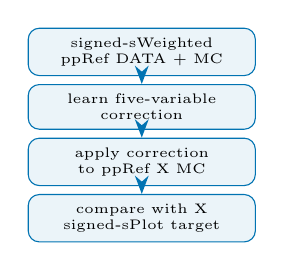
\begin{tikzpicture}[
          node distance=0.10cm,
          box/.style={draw=positive,rounded corners,fill=positive!8,
            text width=2.65cm,minimum height=0.40cm,align=center,font=\tiny},
          arr/.style={-{Stealth},thick,positive}
        ]
          \node[box] (psi) {signed-sWeighted ppRef \psiP DATA + \psiP MC};
          \node[box,below=of psi] (corr) {learn five-variable correction};
          \node[box,below=of corr] (xmc) {apply correction to ppRef X MC};
          \node[box,below=of xmc] (close) {compare with X signed-sPlot target};
          \draw[arr] (psi)--(corr);
          \draw[arr] (corr)--(xmc);
          \draw[arr] (xmc)--(close);
        \end{tikzpicture}
      \end{center}

      \tiny
      Inputs: \texttt{Bcos\_dtheta}, \texttt{Btktkpt}, \texttt{Bchi2Prob},
      \texttt{Btrk2Pt}, \texttt{Btrk1Pt}; correction selection:
      $p_T(B)>7.5$, $|y|<2.4$, \texttt{BQvalue}$<0.15$.
    \end{column}
  \end{columns}

\end{frame}

\begin{frame}{Most variables move closer to the X signed-sPlot target}
  \centering
  \begin{columns}[T]
    \begin{column}{0.32\textwidth}
      \centering
      \includegraphics[width=\textwidth,height=0.34\textheight,keepaspectratio]
      {../XGBoost/output/reweighting/X_pp24_psi2s_R5_rw_v1/transfer_closure_x_splot_v1/variables/Bchi2Prob_transfer_closure.pdf}

      \includegraphics[width=\textwidth,height=0.34\textheight,keepaspectratio]
      {../XGBoost/output/reweighting/X_pp24_psi2s_R5_rw_v1/transfer_closure_x_splot_v1/variables/BtrkPtimb_transfer_closure.pdf}
    \end{column}
    \begin{column}{0.32\textwidth}
      \centering
      \includegraphics[width=\textwidth,height=0.34\textheight,keepaspectratio]
      {../XGBoost/output/reweighting/X_pp24_psi2s_R5_rw_v1/transfer_closure_x_splot_v1/variables/Btrk1Pt_transfer_closure.pdf}

      \includegraphics[width=\textwidth,height=0.34\textheight,keepaspectratio]
      {../XGBoost/output/reweighting/X_pp24_psi2s_R5_rw_v1/transfer_closure_x_splot_v1/variables/Btrk2Pt_transfer_closure.pdf}
    \end{column}
    \begin{column}{0.32\textwidth}
      \centering
      \includegraphics[width=\textwidth,height=0.34\textheight,keepaspectratio]
      {../XGBoost/output/reweighting/X_pp24_psi2s_R5_rw_v1/transfer_closure_x_splot_v1/variables/Bcos_dtheta_transfer_closure.pdf}

      \includegraphics[width=\textwidth,height=0.34\textheight,keepaspectratio]
      {../XGBoost/output/reweighting/X_pp24_psi2s_R5_rw_v1/transfer_closure_x_splot_v1/variables/Btktkpt_transfer_closure.pdf}
    \end{column}
  \end{columns}

  \vfill
  \small\HL{Six variables show point-estimate improvement after transferring the \psiP-derived weights to X MC.}
\end{frame}

\begin{frame}{The remaining variables limit the transfer reliability}
  \begin{columns}[T]
    \begin{column}{0.48\textwidth}
      \centering
      \includegraphics[width=\textwidth,height=0.48\textheight,keepaspectratio]
      {../XGBoost/output/reweighting/X_pp24_psi2s_R5_rw_v1/transfer_closure_x_splot_v1/variables/Btrk1dR_transfer_closure.pdf}
      \small \textbf{\texttt{Btrk1dR}: worsens}\quad $0.1012\to0.1091$
    \end{column}
    \begin{column}{0.48\textwidth}
      \centering
      \includegraphics[width=\textwidth,height=0.48\textheight,keepaspectratio]
      {../XGBoost/output/reweighting/X_pp24_psi2s_R5_rw_v1/transfer_closure_x_splot_v1/variables/BtktkvProb_transfer_closure.pdf}
      \small \textbf{\texttt{BtktkvProb}: small improvement}\quad $0.0472\to0.0393$
    \end{column}
  \end{columns}

  \vspace{0.25em}
  \centering
  \small
  \begin{tabular}{lr}
    \toprule
    Overall diagnostic & Before $\to$ after \\
    \midrule
    Eight-variable mean KS-like distance & $0.1855\to0.1609$ \\
    Variables improved & $7/8$ \\
    \bottomrule
  \end{tabular}

  \vfill
  \HL{The tested \psiP-derived weights do not provide a reliable description of X across all validation variables.}
\end{frame}

\begin{frame}{A new X-based nominal candidate}
  \centering
  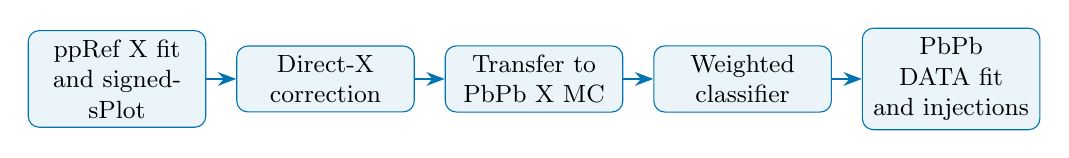
\begin{tikzpicture}[
    box/.style={draw=positive,rounded corners,fill=positive!8,
      minimum height=0.76cm,text width=2.02cm,align=center,font=\small},
    arr/.style={-{Stealth},thick,positive}
  ]
    \node[box] (target) {ppRef X fit\\and signed-sPlot};
    \node[box,right=0.38cm of target] (corr) {Direct-X\\correction};
    \node[box,right=0.38cm of corr] (transfer) {Transfer to\\PbPb X MC};
    \node[box,right=0.38cm of transfer] (ml) {Weighted\\classifier};
    \node[box,right=0.38cm of ml] (fit) {PbPb DATA fit\\and injections};
    \draw[arr] (target)--(corr);
    \draw[arr] (corr)--(transfer);
    \draw[arr] (transfer)--(ml);
    \draw[arr] (ml)--(fit);
  \end{tikzpicture}

  \vspace{0.8em}
  \begin{columns}[T,onlytextwidth]
    \begin{column}{0.70\textwidth}
      \textbf{Why change the route?}
      \begin{itemize}
        \item \psiP-derived correction did not reliably describe X
        \item PbPb \psiP did not provide a usable sPlot target
        \item Use the accepted ppRef X target directly
      \end{itemize}
    \end{column}
  \end{columns}

  \vfill
  \centering\HL{The correction is learned from the ppRef X signed-sPlot target and consumed only within a controlled common support.}
\end{frame}

\begin{frame}{Unrestricted X-target reweighting is unstable}
  \begin{columns}[T]
    \begin{column}{0.52\textwidth}
      \footnotesize
      \textbf{Unrestricted five-variable correction}
      \begin{itemize}
        \item \texttt{Bcos\_dtheta}, \texttt{Btktkpt}, \texttt{Bchi2Prob},
          \texttt{Btrk2Pt}, \texttt{Btrk1Pt}
        \item Fiducial: $7.5<p_T(B)<50$, $|y|<2.4$,
          \texttt{BQvalue}$<0.15$; no controlled input-variable ranges
      \end{itemize}
      \textbf{Assessment of unrestricted X reweighting}
      \begin{tabular}{lr}
        \toprule
        Maximum event weight & $23910.72$ \\
        Weighted-MC $N_{\rm eff}$ & $11.79$ \\
        $\overline{D}$ & $0.1855\to0.3315$ \\
        $D(\texttt{Btrk1dR})$ & $0.1012\to0.5227$ \\
        \bottomrule
      \end{tabular}

      \vspace{0.25em}
      \textbf{Effective sample size:}
      $N_{\rm eff}=(\sum_i w_i)^2/\sum_i w_i^2$, the equivalent number of
      unit-weight events after reweighting.
    \end{column}
    \begin{column}{0.44\textwidth}
      \centering
      \includegraphics[width=\textwidth,height=0.49\textheight,keepaspectratio]
      {../XGBoost/output/reweighting/X_pp24_xsplot_R5_rw_v1/transfer_closure_x_splot_v1/variables/Btrk1dR_transfer_closure.pdf}

      \footnotesize Unrestricted correction strongly distorts \texttt{Btrk1dR}.
    \end{column}
  \end{columns}

  \vfill
  \centering\HL{The unrestricted correction cannot be transferred; common phase-space control is required.}
\end{frame}

\begin{frame}{Correction variable sets}
  \small
  \textbf{Common fiducial:} $7.5<p_T(B)<50$, $|y|<2.4$, \texttt{BQvalue}$<0.15$.

  \vspace{0.45em}
  \centering
  \setlength{\tabcolsep}{6pt}
  \begin{tabular}{lp{10.6cm}}
    \toprule
    Variable set & Reweighting variables \\
    \midrule
    R5 & \texttt{Bcos\_dtheta}, \texttt{Btktkpt}, \texttt{Bchi2Prob},
      \texttt{Btrk2Pt}, \texttt{Btrk1Pt} \\
    R6 & R5 + \texttt{Btrk1dR} \\
    R5v2 & \texttt{Bcos\_dtheta}, \texttt{Btktkpt}, \texttt{Bchi2Prob},
      \texttt{Btrk1Pt}, \texttt{Btrk1dR} \\
    R6v2 & R5v2 + \texttt{Btrk2dR} \\
    \bottomrule
  \end{tabular}

  \vspace{0.8em}
  \begin{columns}[T]
    \begin{column}{0.48\textwidth}
      \textbf{R5 $\to$ R6}\\[0.2em]
      Add \texttt{Btrk1dR} after its closure worsens with R5range.
    \end{column}
    \begin{column}{0.48\textwidth}
      \textbf{R5v2 $\to$ R6v2}\\[0.2em]
      Test track-1-only inputs, then add \texttt{Btrk2dR} explicitly.
    \end{column}
  \end{columns}

  \vfill
  \centering\HL{Variable-set changes and phase-space range changes are tested separately.}
\end{frame}

\begin{frame}{Controlled ranges and tested variants}
  \small
  \begin{columns}[T]
    \begin{column}{0.48\textwidth}
      \textbf{Ranges shared whenever the variable is present}
      \begin{itemize}
        \item \texttt{Bcos\_dtheta} $\in[-1,1]$
        \item \texttt{Bchi2Prob} $\in[0,1]$
        \item \texttt{Btrk1Pt}, \texttt{Btrk2Pt} $\in[0.5,4.5]$
        \item \texttt{Btrk1dR}, \texttt{Btrk2dR} $\in[0,0.5]$
      \end{itemize}

      \vspace{0.3em}
      \textbf{Only \texttt{Btktkpt} changes between range variants}
      \begin{itemize}
        \item R5range, R6range: $[1,10]$
        \item R6range2, R5v2range, R6v2range: $[2,10]$
        \item R5v2range2, R6v2range2: $[2,8]$
      \end{itemize}
    \end{column}
    \begin{column}{0.48\textwidth}
      \centering
      \textbf{Representative outcomes}
      \setlength{\tabcolsep}{4pt}
      \begin{tabular}{lrrr}
        \toprule
        Configuration & max $w$ & $N_{\rm eff}$ & $\overline{D}$ after \\
        \midrule
        R5range & 74.11 & 17106 & 0.0581 \\
        R6range & 951.65 & 2085 & 0.0376 \\
        R6range2 & 16.45 & 34641 & 0.0350 \\
        R5v2range & 15.84 & 32920 & 0.0354 \\
        R6v2range & 38.11 & 28169 & 0.0724 \\
        R5v2range2 & 17.53 & 33836 & 0.0374 \\
        R6v2range2 & 42.33 & 25687 & 0.0738 \\
        \bottomrule
      \end{tabular}

      \vspace{0.4em}
      \textbf{Both track-$dR$ inputs in R6v2range2}\\[0.2em]
      $D(\texttt{Btrk1dR})=0.03552\to0.08319$\\
      $D(\texttt{Btrk2dR})=0.04968\to0.07047$
    \end{column}
  \end{columns}

\end{frame}

\begin{frame}{The second-track angular distance remains mismodelled}
  \begin{columns}[T]
    \begin{column}{0.53\textwidth}
      \centering
      \includegraphics[width=\textwidth,height=0.56\textheight,keepaspectratio]
      {../XGBoost/output/reweighting/X_pp24_xsplot_R6range2_rw_v1/transfer_closure_x_splot_v1/variables/Btrk2dR_transfer_closure.pdf}

      \small R6range2, evaluated within $0<\texttt{Btrk2dR}<0.5$
    \end{column}
    \begin{column}{0.43\textwidth}
      \small
      \textbf{Independent closure check}
      \begin{tabular}{lcc}
        \toprule
        Configuration & $D$ before & $D$ after \\
        \midrule
        R5range & 0.1051 & 0.2014 \\
        R6range2 & 0.0525 & 0.1651 \\
        R5v2range & 0.0493 & 0.1746 \\
        R6v2range & 0.0493 & 0.0840 \\
        \bottomrule
      \end{tabular}

      \vspace{0.6em}
      \begin{itemize}
        \item $\texttt{Btrk2dR}$ is excluded from the eight-variable mean
        \item Adding one or both track-$dR$ inputs does not restore closure
        \item Every tested configuration gives a larger $D(\texttt{Btrk2dR})$
      \end{itemize}
    \end{column}
  \end{columns}

  \vfill
  \centering\HL{The aggregate improvement does not extend to the independent \texttt{Btrk2dR} check.}
\end{frame}

\begin{frame}{Momentum closure improves without resolving track-$dR$}
  \begin{columns}[T]
    \begin{column}{0.48\textwidth}
      \centering
      \textbf{R5range: includes \texttt{Btrk2Pt}}\\[0.2em]
      \includegraphics[width=\textwidth,height=0.48\textheight,keepaspectratio]
      {../XGBoost/output/reweighting/X_pp24_xsplot_R5range_rw_v1/transfer_closure_x_splot_v1/variables/Btrk2Pt_transfer_closure.pdf}

      \small $D(\texttt{Btrk2Pt}):\ 0.239176\to0.031423$
    \end{column}
    \begin{column}{0.48\textwidth}
      \centering
      \textbf{R5v2range: excludes \texttt{Btrk2Pt}}\\[0.2em]
      \includegraphics[width=\textwidth,height=0.48\textheight,keepaspectratio]
      {../XGBoost/output/reweighting/X_pp24_xsplot_R5v2range_rw_v1/transfer_closure_x_splot_v1/variables/Btrk2Pt_transfer_closure.pdf}

      \small $D(\texttt{Btrk2Pt}):\ 0.106097\to0.031412$
    \end{column}
  \end{columns}

  \vspace{0.25em}
  \small
  \textbf{Contrast:} \texttt{Btrk2Pt} improves strongly whether it is a correction input or
  an independent check, while \texttt{Btrk2dR} worsens in all tested configurations.

  \vfill
  \centering\HL{R6range2 is a pragmatic stability--closure compromise; no tested variant resolves \texttt{Btrk2dR}.}
\end{frame}

\begin{frame}[label=p18]{Transfer is restricted to a common phase space}
  \begin{tikzpicture}[remember picture,overlay]
    \node[anchor=north west] at ([xshift=0.802cm,yshift=-0.997cm]current page.north west) {%
      \includegraphics[width=8.64cm,height=7.38cm,keepaspectratio]
      {../XGBoost/output/reweighting/X_pp24_xsplot_R6range2_rw_v1/ppref_pbpb_mc_comparison_v1/common_fiducial_in_r6range2_support/variables/BtrkPtimb_ppref_vs_pbpb_unweighted.pdf}%
    };
  \end{tikzpicture}
  \vspace{-1.2em}
  \begin{columns}[T]
    \begin{column}{0.70\textwidth}
      \mbox{}

    \end{column}
    \begin{column}{0.27\textwidth}
      \hspace{-0.5\textwidth}%
      \begin{minipage}[t]{1.5\textwidth}
        \footnotesize
        \textbf{1. Transfer domain}\\[0.2em]
        Learn inside ppRef R6range2 support. Apply with tighter PbPb:
        $10<\texttt{Bpt}<50$, $|\texttt{By}|<1.6$, \texttt{BQvalue}$<0.15$.

        \vspace{0.3em}
        \textbf{2. MC-domain baseline}\\[0.2em]
        Compare unweighted ppRef/PbPb MC. Adding full support, including
        \texttt{Btktkpt}$\in[2,10]$, changes mean $\overline D$ from 0.0943 to 0.0843.

        \vspace{0.3em}
        \textbf{3. Apply contract}\\[0.2em]
        Reweight 32,160 in-support events; keep 22,908 outside at unity and
        exclude them downstream.
      \end{minipage}
    \end{column}
  \end{columns}
\end{frame}

\begin{frame}{Weighted and unweighted classifiers define the fit inputs}
  \footnotesize
  \begin{columns}[T]
    \begin{column}{0.48\textwidth}
      \textbf{Shared training definition}
      \begin{itemize}
        \item Background: PbPb DATA, \texttt{Bmass}$\in[3.75,3.80]\cup[3.95,4.00]$ GeV
        \item Candidate-level 75/25 split; common support
      \end{itemize}
    \end{column}
    \begin{column}{0.48\textwidth}
      \textbf{Only the signal model changes}
      \begin{itemize}
        \item Weighted: transferred correction on PbPb X MC
        \item Unweighted: unit-weight PbPb X MC
        \item Same fit workflow consumes both scored samples
      \end{itemize}
    \end{column}
  \end{columns}

  \vspace{0.15em}
  \textbf{Eight shared inputs:}
  \texttt{Bchi2Prob}, \texttt{Btrk1dR}, \texttt{BtrkPtimb}, \texttt{Btrk1Pt},
  \texttt{Btrk2Pt}, \texttt{BtktkvProb}, \texttt{Bcos\_dtheta}, \texttt{Btktkpt}.

  \vspace{0.3em}
  \centering
  \begin{tabular}{lccc}
    \toprule
    Classifier & signal weighting & train AUC & test AUC \\
    \midrule
    Weighted signal & transferred event weights & 0.8777 & 0.8391 \\
    Unit signal & unit event weights & 0.9115 & 0.8958 \\
    \bottomrule
  \end{tabular}

  \vspace{0.3em}
  \textbf{Interpretation boundary:} the classifiers see different signal distributions;
  a higher MC AUC may absorb DATA--MC mismatch and does not select the physical model.

  \vfill
  \centering\HL{AUC and SHAP describe model response; the decision requires observed spectra and injection tests.}
\end{frame}

\begin{frame}[label=p20]{Observed data after the unweighted classifier}
  \begin{columns}[T,onlytextwidth]
    \begin{column}{0.62\textwidth}
      \centering
      \includegraphics[width=1.10\textwidth,height=0.66\textheight,keepaspectratio]
      {../Analysis_CODES/fitER/results/PbPb_H012_template_ml_matrix_narrow_range/unweighted_ml_xeff20/background_fit.pdf}
    \end{column}
    \begin{column}{0.36\textwidth}
      \footnotesize
      \textbf{Selected spectrum}
      \begin{itemize}
        \item 20\% weighted-reference X efficiency
        \item 4087 DATA candidates
        \item \texttt{Bmass}: 3.80--3.94 GeV
        \item Smooth second-order background
      \end{itemize}
      \textbf{Fit quality}
      \begin{itemize}
        \item status $=0$
        \item covQual $=3$
        \item $\chi^2/{\rm ndf}=0.771$
      \end{itemize}
    \end{column}
  \end{columns}

  \vfill
  \centering\HL{No narrow X peak is clearly visible; a smooth background-only model adequately describes this selected spectrum.}
\end{frame}

\begin{frame}[label=p21]{Observed data after the weighted classifier}
  \begin{columns}[T,onlytextwidth]
    \begin{column}{0.62\textwidth}
      \centering
      \includegraphics[width=1.10\textwidth,height=0.66\textheight,keepaspectratio]
      {../Analysis_CODES/fitER/results/PbPb_H012_template_ml_matrix_narrow_range/weighted_ml_xeff20/background_fit.pdf}
    \end{column}
    \begin{column}{0.36\textwidth}
      \footnotesize
      \textbf{Selected spectrum}
      \begin{itemize}
        \item 20\% weighted-reference X efficiency
        \item 2799 DATA candidates
        \item \texttt{Bmass}: 3.80--3.94 GeV
        \item Smooth second-order background
      \end{itemize}
      \textbf{Fit quality}
      \begin{itemize}
        \item status $=0$
        \item covQual $=3$
        \item $\chi^2/{\rm ndf}=0.662$
      \end{itemize}
    \end{column}
  \end{columns}

  \vfill
  \centering\HL{The weighted classifier also yields no clearly visible narrow X peak in the observed spectrum.}
\end{frame}

\begin{frame}{The absence of a visible peak is not a transfer test by itself}
  \small
  \centering
  \begin{tabular}{lrrrr}
    \toprule
    & \multicolumn{4}{c}{Weighted-reference X efficiency} \\
    \cmidrule(lr){2-5}
    Classifier & 20\% & 30\% & 40\% & 50\% \\
    \midrule
    Unweighted: DATA candidates & 4087 & 10765 & 23422 & 43273 \\
    Unweighted: $\chi^2/{\rm ndf}$ & 0.771 & 0.979 & 0.981 & 0.762 \\
    Weighted: DATA candidates & 2799 & 7742 & 16983 & 31399 \\
    Weighted: $\chi^2/{\rm ndf}$ & 0.662 & 1.217 & 0.917 & 0.569 \\
    \bottomrule
  \end{tabular}

  \vspace{0.65em}
  \begin{itemize}
    \item All eight background-only fits converge
    \item No clearly visible narrow X peak
    \item Smooth background gives an acceptable description
  \end{itemize}

  \vfill
  \centering\HL{A leading explanation for the absent peak is residual mismatch between the reweighted MC and the signal-variable distributions.}
\end{frame}

\begin{frame}[label=p23]{A matched-signal injection tests the current workflow}
  \footnotesize
  \textbf{Validation question}
  \begin{enumerate}
    \item Generate pseudo-data with signal-variable distributions matching the current X MC.
    \item Apply the current classifier selection and \texttt{Bmass} fit workflow.
    \item Test whether the injected narrow signal peak and yield are recovered.
  \end{enumerate}

  \vspace{0.2em}
  \begin{columns}[T]
    \begin{column}{0.45\textwidth}
      \textbf{Signal-yield estimate}
      \[
        N_X^{\rm after}=N_{\psi}^{\rm raw}\times1.08\times
        \frac{\epsilon_X^{\rm score}}{\epsilon_{\psi}^{\rm score}}.
      \]
      \begin{itemize}
        \item $N_{\psi}^{\rm raw}$ from eight accepted PbPb DATA fits
        \item Expected yield evaluated after each score cut
      \end{itemize}
    \end{column}
    \begin{column}{0.51\textwidth}
      \centering
      \textbf{Expected signal yields}
      \setlength{\tabcolsep}{4pt}
      \begin{tabular}{crr}
        \toprule
        X efficiency & weighted & unweighted \\
        \midrule
        20\% & $90.0\pm22.2$ & $67.6\pm17.7$ \\
        30\% & $114.4\pm32.3$ & $137.2\pm27.9$ \\
        40\% & $193.5\pm73.2$ & $184.5\pm40.8$ \\
        50\% & $235.8\pm63.2$ & $212.7\pm55.5$ \\
        \bottomrule
      \end{tabular}
    \end{column}
  \end{columns}

  \vspace{0.35em}
  \textbf{Fast-test assumptions:}
  pre-score acceptance--efficiency ratio $=1$; prompt-fraction ratio $=1$;
  only the \psiP fit statistical uncertainty is propagated.
\end{frame}

\begin{frame}[label=p24]{Matched-model injections recover the assumed signal}
  \begin{columns}[T,onlytextwidth]
    \begin{column}{0.66\textwidth}
      \centering
      \raisebox{-0.2\height}{%
        \includegraphics[width=1.31\textwidth,height=0.696\textheight,keepaspectratio]
        {../Analysis_CODES/fitER/results/PbPb_H011_x_ratio_injection_fast_toys/toy_sensitivity_summary.pdf}%
      }
    \end{column}
    \begin{column}{0.32\textwidth}
      \footnotesize
      \textbf{Fast-test design}
      \begin{itemize}
        \item Asimov fits at the central yield and $\pm1\sigma_{\psi}$
        \item 200 toys with the central signal injection
        \item 200 background-only toys
        \item Generation and fit use matching signal models
      \end{itemize}
      \textbf{Observed in toys}
      \begin{itemize}
        \item Median expected $Z$: 2.66--4.15
        \item Central Asimov bias: $-0.8\%$ to $-3.3\%$
        \item Background-only: 12--43\% failure; 71.5--88\% boundary
      \end{itemize}
    \end{column}
  \end{columns}

  \vfill
  \centering\HL{Matched-signal sensitivity does not validate the ppRef-to-PbPb transfer in data.}
\end{frame}

\begin{frame}[label=p25]{Template and classifier choices do not yet define an optimum}
  \begin{columns}[T,onlytextwidth]
    \begin{column}{0.66\textwidth}
      \centering
      \raisebox{-0.2\height}{%
        \includegraphics[width=1.24\textwidth,height=0.696\textheight,keepaspectratio]
        {../Analysis_CODES/fitER/results/PbPb_H012_template_ml_matrix_narrow_range/toy_sensitivity_matrix_summary.pdf}%
      }
    \end{column}
    \begin{column}{0.32\textwidth}
      \footnotesize
      \textbf{Matching-template matrix}
      \begin{itemize}
        \setlength{\itemsep}{0.1em}
        \item Each template $\times$ classifier: central and $\pm1\sigma_{\psi}$ Asimov fits
        \item 200 central-injection + 200 background-only toys
        \item Median $Z$: 2.52--5.01
      \end{itemize}
      \textbf{Remaining limitations}
      \begin{itemize}
        \setlength{\itemsep}{0.1em}
        \item Mean failure change: $-0.0275$
        \item No systematic covQual/boundary gain
        \item 7 central recovery warnings
      \end{itemize}
    \end{column}
  \end{columns}

  \vfill
  \centering\HL{Expected sensitivity depends jointly on template, classifier, and injected yield; no final model or working point is established.}
\end{frame}

\begin{frame}[label=p26]{Summary and Outlook}
  \small
  \begin{center}
    \renewcommand{\arraystretch}{1.22}
    \begin{tabular}{p{3.2cm}p{5.0cm}p{5.0cm}}
      \toprule
      Question & Established & Remaining limitation \\
      \midrule
      Extreme weights & Range control restores $N_{\rm eff}$ & \\
      Variables/ranges & A working configuration & Not optimal \\
      \texttt{Btrk1dR}/\texttt{Btrk2dR} & & Failure persists across variants \\
      Region transfer & Explicit extrapolation is excluded & No PbPb DATA closure \\
      Observed spectra & & No clearly visible narrow X peak \\
      Injection checks & ML is working & \\
      \bottomrule
    \end{tabular}
  \end{center}

  \vspace{0.25em}
  \raggedright
  \textbf{Possible ways forward}
  \begin{enumerate}
    \item Test ppRef \psiP correction transfer within common support.
    \item Compare variables/ranges with common validation gates.
    \item Explore additional potentially useful input variables.
  \end{enumerate}
\end{frame}

\begin{frame}[label=p27]{\strut}
  \centering
  \vfill
  \makebox[\textwidth][c]{%
    \begin{beamercolorbox}[wd=0.68\textwidth,sep=1.2em,center,rounded=true,shadow=true]{block body}
      {\LARGE\bfseries Thanks for listening!}\par
      \vspace{1.0em}
      {\large Reporter: Lekai Yao}\par
      \vspace{0.45em}
      {\large 2026.8.5}
    \end{beamercolorbox}%
  }
  \vfill
\end{frame}

\end{document}
